\section{Available equipements}
Debugging Linux is a challenging task which requires a good preparation.
\subsection{Hardware}


\subsubsection{Beagle Bone Black Wireless} 
The evolution of beaglebone black which adds wireless support (WIFI, Bluetooth) and fast linux boot (\textbf{Figure \ref{Beaglebone black wireless}}). 
		\begin{figure}[H]
			\centering
        	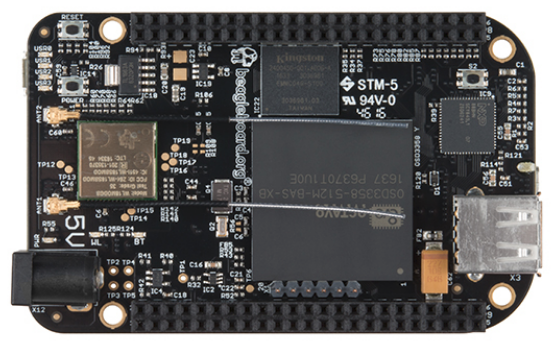
\includegraphics[scale=0.25]{img/mean/beaglebone-black-wireless.png}
        	\caption{Beaglebone black wireless}
        	\label{Beaglebone black wireless}
    	\end{figure}
\begin{center}
\textbf{\color{red}Hardware specifications} 
A datasheet is available at : {\color{blue}\url{https://www.alliedelec.com/m/d/5505861ee370de1c82065dcc7bc77b0c.PDF}}.
\end{center}

\subsubsection{Raspberry PI 3 B+}
The lastest version as this time of writing with enhanced processor and ethernet speed (\textbf{Figure \ref{Raspberry PI 3}}).
		\begin{figure}[H]
			\centering
        	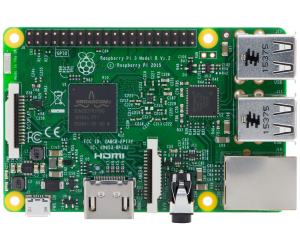
\includegraphics[scale=0.32]{img/mean/rpi3.png}
        	\caption{Raspberry PI 3}
        	\label{Raspberry PI 3}
    	\end{figure}
    	
\begin{center}	
\textbf{\color{red}Hardware specifications} 
A datasheet is available at : {\color{blue}\url{https://static.raspberrypi.org/files/product-briefs/Raspberry-Pi-Model-Bplus-Product-Brief.pdf}}.
\end{center}


\subsubsection{stm32f407 Board : } (\textbf{Figure \ref{stm32f407 Board}})  specifications are available at : {\color{blue}\url{https://www.st.com/content/ccc/resource/technical/document/user_manual/70/fe/4a/3f/e7/e1/4f/7d/DM00039084.pdf/files/DM00039084.pdf/jcr:content/translations/en.DM00039084.pdf}}
		\begin{figure}[H]
			\centering
        	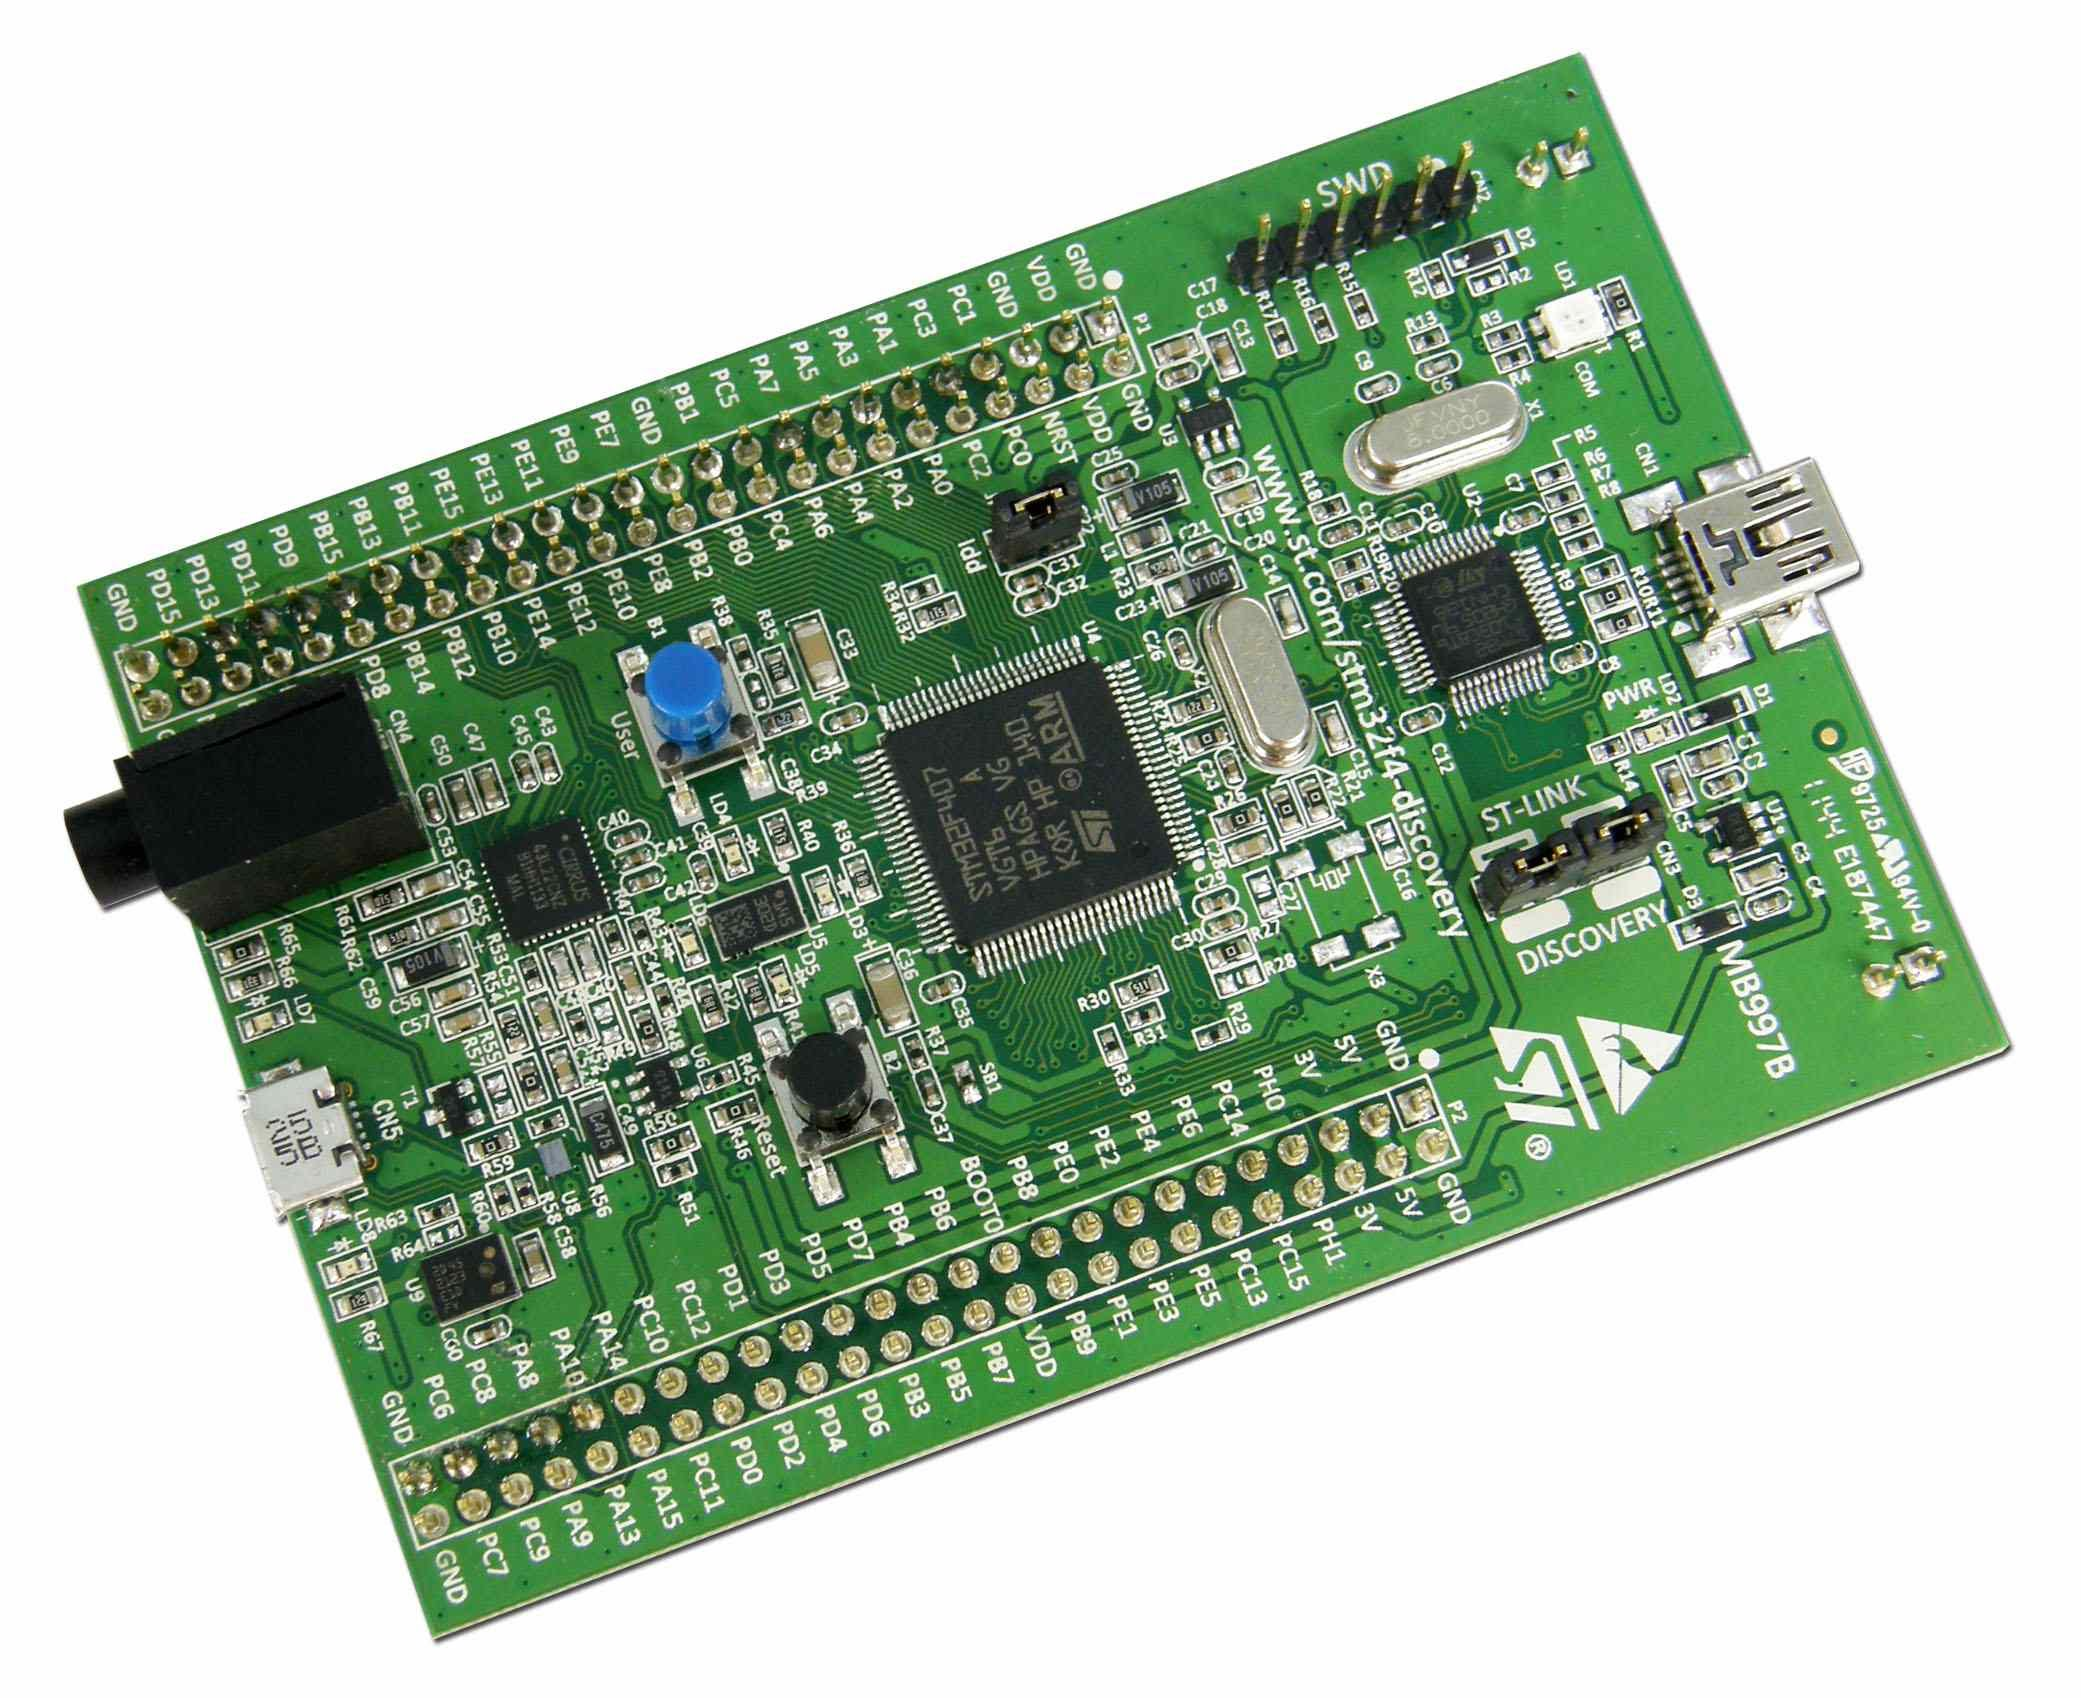
\includegraphics[scale=0.08]{img/mean/stm-32.jpg}
        	\caption{stm32f407 Board}
        	\label{stm32f407 Board}
    	\end{figure}


\subsubsection{AT32UC3C-EK Board : } (\textbf{Figure \ref{AT32UC3C Board}}) see the following link for spefications :  {\color{blue}\url{http://www.farnell.com/datasheets/1511964.pdf}} 
		\begin{figure}[H]
			\centering
        	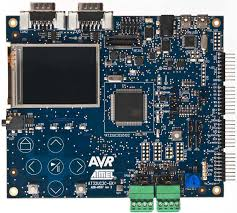
\includegraphics[scale=0.40]{img/mean/avr32.jpeg}
        	\caption{AT32UC3C Board}
        	\label{AT32UC3C Board}
    	\end{figure}

\subsubsection{ARM-USB-TINY-H JTAG Adapter : }  OpenOCD debugging interface adapter (see \textbf{Figure \ref{ARM-USB-TINY-H}}).
		\begin{figure}[H]
			\centering
        	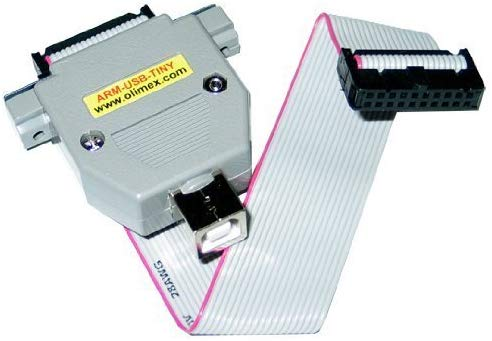
\includegraphics[scale=0.25]{img/mean/arm-usb-tiny-h.jpg}
        	\caption{ARM-USB-TINY-H}
        	\label{ARM-USB-TINY-H}
    	\end{figure}
{\color{blue}\url{https://www.olimex.com/Products/ARM/JTAG/_resources/ARM-USB-TINY_and_TINY_H_manual.pdf}}
\subsection{Software}
\subsubsection{pycharm}
Pycharm is a python IDE, which makes developement fast.
\subsubsection{Eclipse C/C++}
Code examples were written maily in C, Eclipse C/C++ was helpful. 